\documentclass[a4paper,UKenglish,cleveref, autoref, thm-restate]{template/lipics-v2021}
%This is a template for producing LIPIcs articles.
%See lipics-v2021-authors-guidelines.pdf for further information.
%for A4 paper format use option "a4paper", for US-letter use option "letterpaper"
%for british hyphenation rules use option "UKenglish", for american hyphenation rules use option "USenglish"
%for section-numbered lemmas etc., use "numberwithinsect"
%for enabling cleveref support, use "cleveref"
%for enabling autoref support, use "autoref"
%for anonymousing the authors (e.g. for double-blind review), add "anonymous"
%for enabling thm-restate support, use "thm-restate"
%for enabling a two-column layout for the author/affilation part (only applicable for > 6 authors), use "authorcolumns"
%for producing a PDF according the PDF/A standard, add "pdfa"

\pdfoutput=1 %uncomment to ensure pdflatex processing (mandatatory e.g. to submit to arXiv)
\hideLIPIcs  %uncomment to remove references to LIPIcs series (logo, DOI, ...), e.g. when preparing a pre-final version to be uploaded to arXiv or another public repository

\bibliographystyle{plainurl}% the mandatory bibstyle

\usepackage[activate={true,nocompatibility},final,tracking=true,kerning=true,spacing=true,factor=1100]{microtype}

\usepackage{tikz}
\usepackage{float}
\usepackage{pgfplots}
\usepgfplotslibrary{colorbrewer}

\title{Report: Engineering a Sorting Algorithm}

\author{Stefan Tobias Koch}{Karlsruhe Institute of Technology, Germany}{stefan.koch@student.kit.edu}{}{}

\authorrunning{S. T. Koch}

\nolinenumbers

\begin{document}
	
	\maketitle
	
	\section{General Approach}
	
	The approach we take to implement an efficient sorting algorithm follows the recommendation of using a recursive radix sort that switches to Robin Hood sort for sufficiently small chunks of data.
	
	Our radix sort exclusively uses two bins to avoid the counting phase, requiring only a single pass over the data.
	
	Our Robin Hood sort uses linear probing for collision resolution, shifting elements when needed to insert an element between two occupied slots.
	This maintains a sorted order within the auxiliary array.
	
	\section{Optimizations}
	
	All experiments are repeated until either 10 seconds have elapsed or the experiment has been repeated 10,000 times.
	Unless otherwise stated, 10,000,000 uniformly randomly distributed elements are sorted.
	This is the input size to which we primarily optimize and tune our algorithm to.
	
	\subsection{Eliminating memory allocations}
	
	Preliminary experiments show, that it appears significantly faster to exclusively rely on radix sort.
	This is caused by our naive implementation of Robin Hood sort requiring expensive memory allocations for each invocation to store the auxiliary array. Since Robin Hood sort invocations represent leaves in the recursion tree, there are potentially numerous.
	
	The solution is reusing a (thread-local) static buffer as the auxiliary array.
	This buffer must be cleaned between uses, which can simply be done when the elements are being written back to the primary data structure.
	This design suggests two tuning parameters: the maximum size of a bin at which the algorithm switches to Robin Hood sort $r$ and the overallocation factor of the auxiliary buffer $m$.
	
	\cref{fig:pt} shows a two-dimensional parameter tuning of these parameters.
	$m$ offers a trade-off between less collisions with high $m$ and shorter linear scans over the buffer with low $m$.
	The results are both highly peculiar and interesting.
	The theoretically minimal $m$ of 2 (which assures that shifting elements following a collision always succeeds) appears optimal, suggesting the linear scan to be the dominant factor here.
	Interestingly, exclusively using radix sort still beats even the best configuration utilizing Robin Hood sort, while at the same time performance improves for Robin Hood sort with increasing $r$, meaning the sooner it starts, the better.
	If the observed trend continues it seems likely that when the input data and $r$ get large enough, there will be a point of inversion where using Robin Hood sort beats exclusively relying on radix sort.
	We will be using the optimal configuration with $m=2$ and $r=10^6$ for future experiments along with the pure radix sort variant.

	\begin{figure}[h]
		\centering
		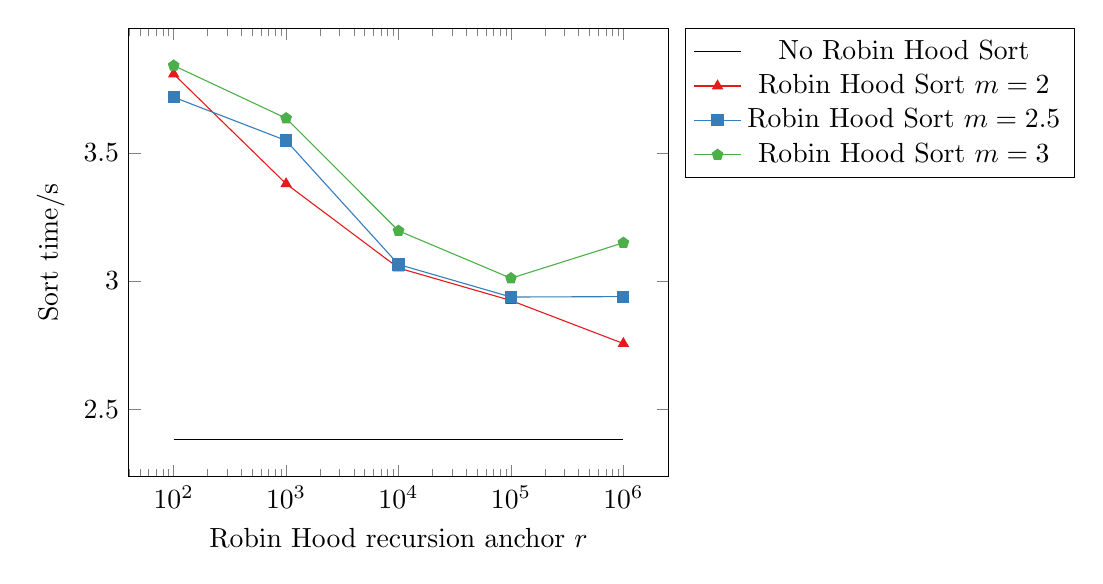
\begin{tikzpicture}
			\begin{axis}[
				xmode=log,
				xlabel=Robin Hood recursion anchor $r$,
				ylabel=Sort time/s,
				legend pos=outer north east
			]
				\addplot[
					color=black,
					domain=100:1000000,
				] {
					2.382720160
				};
				\addplot[
					color=Set1-A,
					mark=triangle*,
				]
				coordinates {
					(100,     3.807953066)
					(1000,    3.379549833)
					(10000,   3.050851925)
					(100000,  2.924031075)
					(1000000, 2.756095875)
				};
				\addplot[
					color=Set1-B,
					mark=square*,
				]
				coordinates {
					(100,     3.717625633)
					(1000,    3.548318400)
					(10000,   3.064629300)
					(100000,  2.937659400)
					(1000000, 2.939171300)
				};
				\addplot[
					color=Set1-C,
					mark=pentagon*
				]
				coordinates {
					(100,     3.841011466)
					(1000,    3.635475666)
					(10000,   3.196108600)
					(100000,  3.010947250)
					(1000000, 3.149276650)
				};
				\legend{No Robin Hood Sort, Robin Hood Sort $m=2$, Robin Hood Sort $m=2.5$, Robin Hood Sort $m=3$}
			\end{axis}
		\end{tikzpicture}
		\caption{Plot comparing different configurations of the algorithm. The Robin Hood recursion anchor is the maximum bin size at which the radix sort recursion ends with a Robin Hood sort.}
		\label{fig:pt}
	\end{figure}
	
	We compare the scaling behavior of three variants in \cref{fig:comp}.
	In ``max buffer Robin Hood sort``, each invocation of Robin Hood sort uses the entirety of the allocated auxiliary array, independently of the actual size of the data to sort.
	While this generally lessens the chances of collisions, the linear scans of fixed size add constant overhead that heavily dominates the runtime of the complete algorithm for small inputs.
	Other than that we see slightly superlinear scaling as is to be expected with the Robin Hood sort variant lacking behind the pure radix sort variant but narrowing the gap with growing input sizes.
	
	\begin{figure}[h]
		\centering
		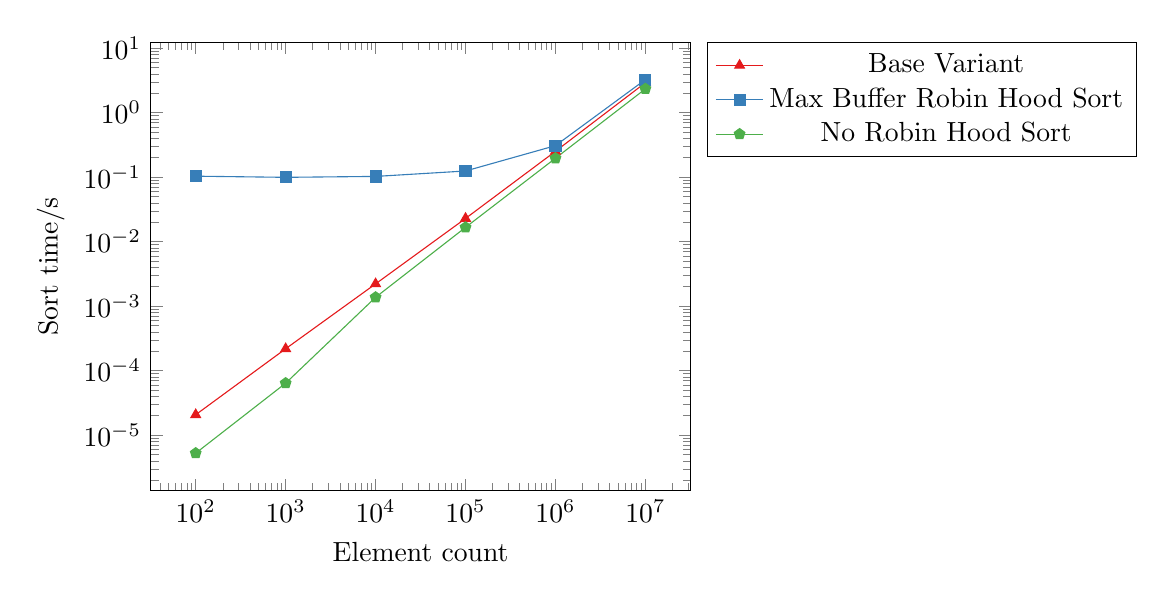
\begin{tikzpicture}
			\begin{axis}[
				xmode=log,
				ymode=log,
				xlabel=Element count,
				ylabel=Sort time/s,
				legend pos=outer north east
			]
				\addplot[
					color=Set1-A,
					mark=triangle*,
				]
				coordinates {
					(100,      0.000020746)
					(1000,     0.000218623)
					(10000,    0.002217252)
					(100000,   0.022902563)
					(1000000,  0.251721767)
					(10000000, 2.915275750)
				};
				\addplot[
					color=Set1-B,
					mark=square*,
				]
				coordinates {
					(100,      0.103543187)
					(1000,     0.099439755)
					(10000,    0.102730047)
					(100000,   0.124656567)
					(1000000,  0.308068244)
					(10000000, 3.256186157)
				};
				\addplot[
					color=Set1-C,
					mark=pentagon*,
				]
				coordinates {
					(100,      0.000005258)
					(1000,     0.000063989)
					(10000,    0.001372270)
					(100000,   0.016661678)
					(1000000,  0.196576704)
					(10000000, 2.338274811)
				};
				\legend{Base Variant, Max Buffer Robin Hood Sort, No Robin Hood Sort}
			\end{axis}
		\end{tikzpicture}
		\caption{Comparing different variants at varying input sizes.}
		\label{fig:comp}
	\end{figure}
	
	\subsection{Unrolling Recursion}
	\label{sec:ur}
	
	For radix sort, making the bit position to sort by a compile-time constant gives the compiler the ability to inline the recursive calls (among other optimizations), potentially unrolling the entire recursion at the cost of a larger binary and the possibility of more instruction cache misses.
	
	The observed benefit is slight but noticeable.
	This step also serves as a prerequisite for \cref{sec:mmt}.
	
	\subsection{Minimizing Memory Traffic}
	\label{sec:mmt}
	
	The basic idea is to parameterize subroutines on the smallest possible data type that encompasses all relevant bits for its invocation.
	Since radix sort occurs entirely in-place, it seems unlikely that truncating higher order bits can reasonably be utilized within it.
	Using smaller data types to swap elements yielded no measurable performance difference.
	This leaves Robin Hood sort as the only viable candidate.
	The idea here is to use a smaller data type for the auxiliary array, allowing its space to be used more efficiently and decreasing collision count.
	However, in practice switching to Robin Hood sort always occurs with $>32$ bits remaining relevant, meaning this optimization yields no behavioral difference.
	
	\subsection{Parallelization}
	
	We attempt two approaches to parallelization.
	In the first, we store each node in the recursion tree as a job in a stack shared among the processors.
	A thread always tries to continue one of its own recursive invocations to improve cache efficiency.
	One downside to this approach is a start-up phase when not many jobs are available, leaving most processors idle.
	\footnote{This approach is not compatible with the optimization found in \cref{sec:ur} and subsequently \cref{sec:mmt}.}
	
	In the second approach, we utilize the partitioning, sorting one chunk of data on every thread and merging the results recursively and in parallel from the bottom up.
	One benefit of this approach is the avoidance of false sharing among the threads in the individual sort phase.
	Unfortunately, the in-place merging of multiple non-contiguous blocks of sorted data has proven to be prohibitively expensive, making this approach not practicable.
	
	Two variants of the first approach yield the speedups found in \cref{fig:par}.
	
	\begin{figure}[h]
		\centering
		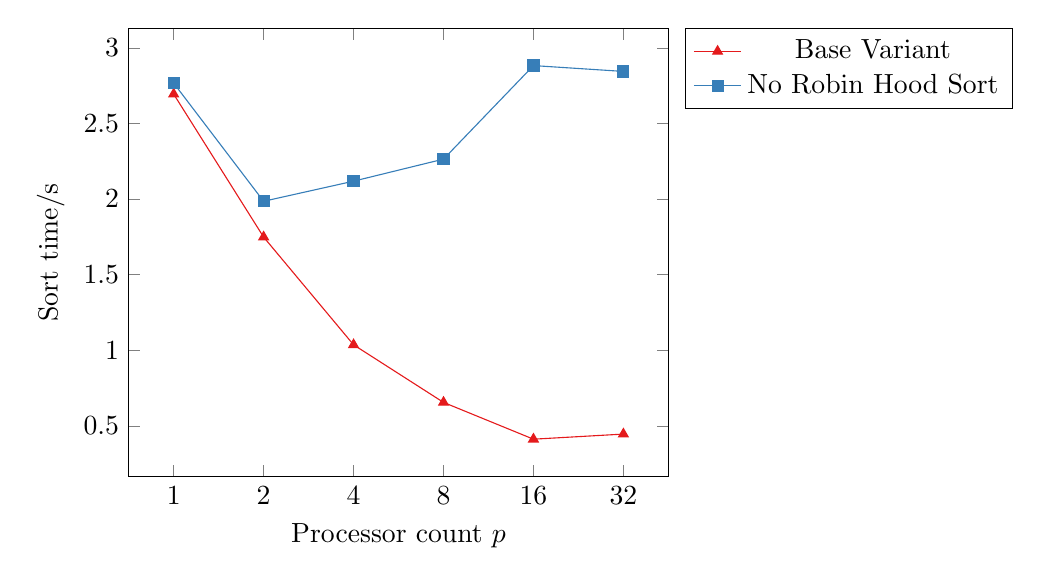
\begin{tikzpicture}
			\begin{axis}[
				xmode=log,
				log basis x=2,
				xticklabels={0, 1, 2, 4, 8, 16, 32},
				xlabel=Processor count $p$,
				ylabel=Sort time/s,
				legend pos=outer north east
			]
				\addplot[
					color=Set1-A,
					mark=triangle*,
				]
				coordinates {
					(1,  2.693712787)
					(2,  1.748531833)
					(4,  1.036100125)
					(8,  0.655303477)
					(16, 0.412009663)
					(32, 0.445747260)
				};
				\addplot[
					color=Set1-B,
					mark=square*,
				]
				coordinates {
					(1,  2.766381412)
					(2,  1.985146136)
					(4,  2.118121840)
					(8,  2.264000155)
					(16, 2.882427228)
					(32, 2.843830300)
				};
				\legend{Base Variant, No Robin Hood Sort}
			\end{axis}
		\end{tikzpicture}
		\caption{Comparing parallel scaling behavior of different variants.}
		\label{fig:par}
	\end{figure}
	
	The base variant sees a total speedup of 6.5 with $p=16$.
	The drop at $p=32$ is caused by not all processors receiving jobs, due to the high $r$ resulting in few total recursion steps.
	The pure radix sort variant scales incredibly poorly, which is likely caused by the high number of very small jobs that result in high contention on the job stack.
	These results validate the use of Robin Hood sort and suggest that renewed parameter tuning with $p=32$ might provide interesting results, although I will refrain from straining the page limit any further.

	\appendix
	
\end{document}
